\documentclass[12pt]{article}
\usepackage{graphicx}
\graphicspath{ {./img/} }
\begin{document}
\section*{Authentication, Authorization methods}
\subsection*{Learning objectives}
\begin{itemize}
    \item the strengths and weaknesses of the seven fundamental authentication schemes.
    \item the principles of zero knowledge password proofs(schema A5).
    \item federated identitiesas strict separation between identity providersand service providers
    \item SAML 2.0 assertionsin    portable identitiesand the related XML security mechanismswith which SAML guarantees trustworthiness and privacy.
    \item OAuth 2.0roles of client,  resource owner,  authorization serverand resource serverand the top level processes by which a client can get access to a protected resource.
    \item You know that currently trustworthiness and privacy of the OAuth 2.0protocol is exclusively based on Transport Layer Security(TLS).
\end{itemize}

\subsection*{Authentication Authorization Accounting}
\subsubsection*{Identification}
I am: "Username"
\subsubsection*{Authentication}
Prove, that I am "Username"
\subsubsection*{Authorization}
Grant access for "Username"
\subsubsection*{Accounting}
Log what "Username" has document
\subsection*{Fundamental Authentication Schemes}
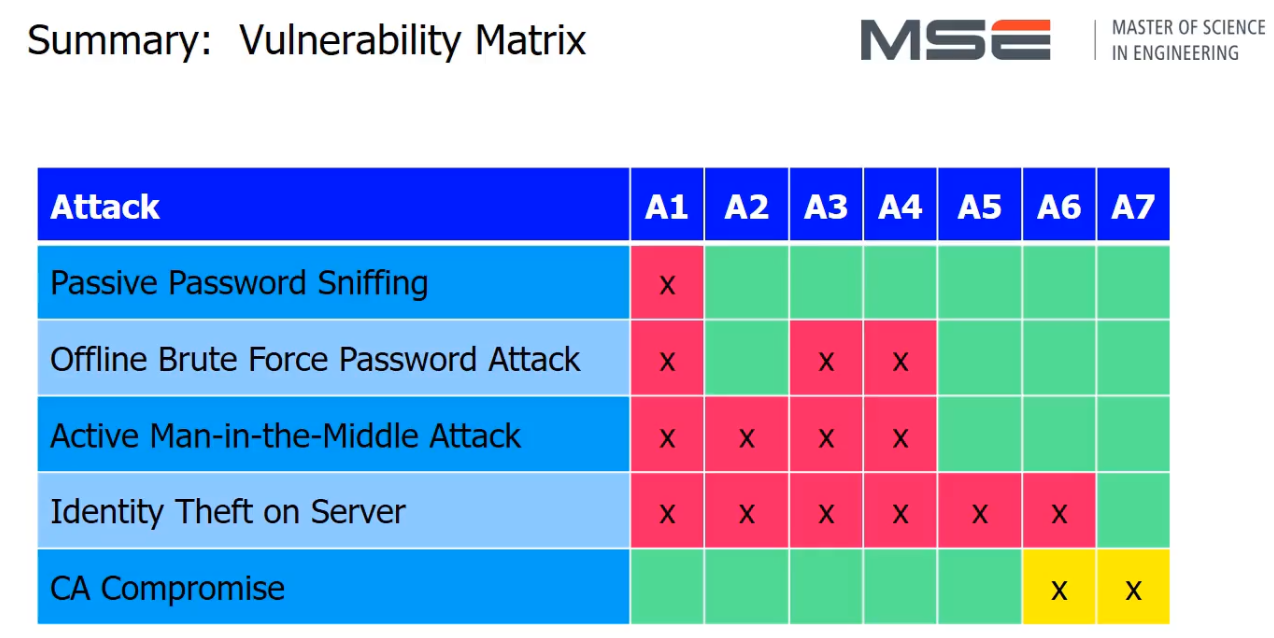
\includegraphics[width=\textwidth]{VulnerabilityMatrix.png}
\subsubsection*{Basic Authentication}
Username + password

Cheap, very easily deploied, easy to use
\subsubsection*{One time password}
For example use SecureID to generate passwords

Is vulnerable to MIM

Tokens need to be ordered and are expensive on user and serverside.
\subsubsection*{Challenge response}
Server sends a challenge, user applies a one way function to the challenge and sends the response to the server.

A function can be applying his password to the challenge.
\begin{itemize}
    \item No secrets are openly transmitted
    \item Is vulnerable to MIM
    \item Password still needs to be strong.
    \item If password is weak, it can be brute forced.
    \item Cheap
    \item Why are they used -> Authentication over unsecure channel without transmitting the secret.
\end{itemize}
How does it work?

Server sends random value (Rs) to user. User creates hash using (Rs), a new random value (Ru) and his password.
(Ru) and generated hash are sent to server. Server applies same hash function and compares hash.

Kerberos is another example (Used in windows)

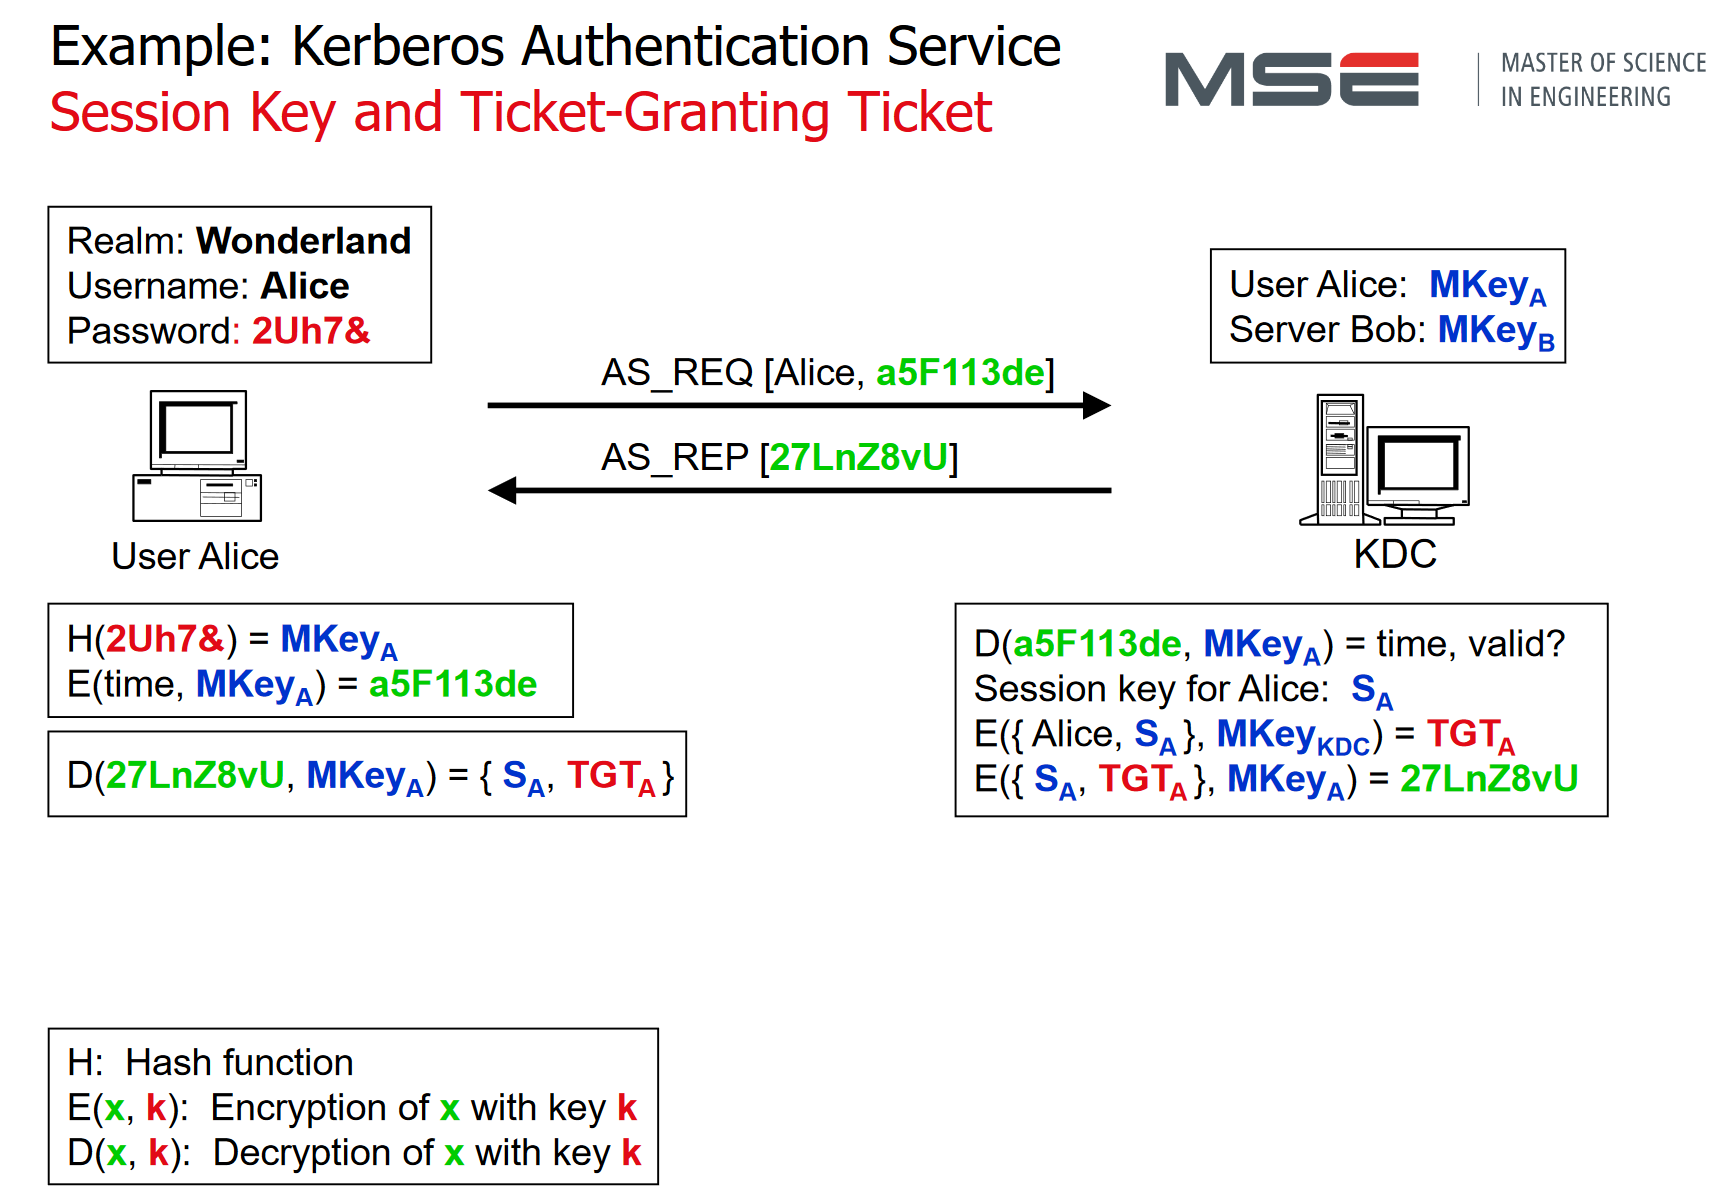
\includegraphics[width=\textwidth]{KerberosAuthenticationService.png}

Dignital signatures can be used as well

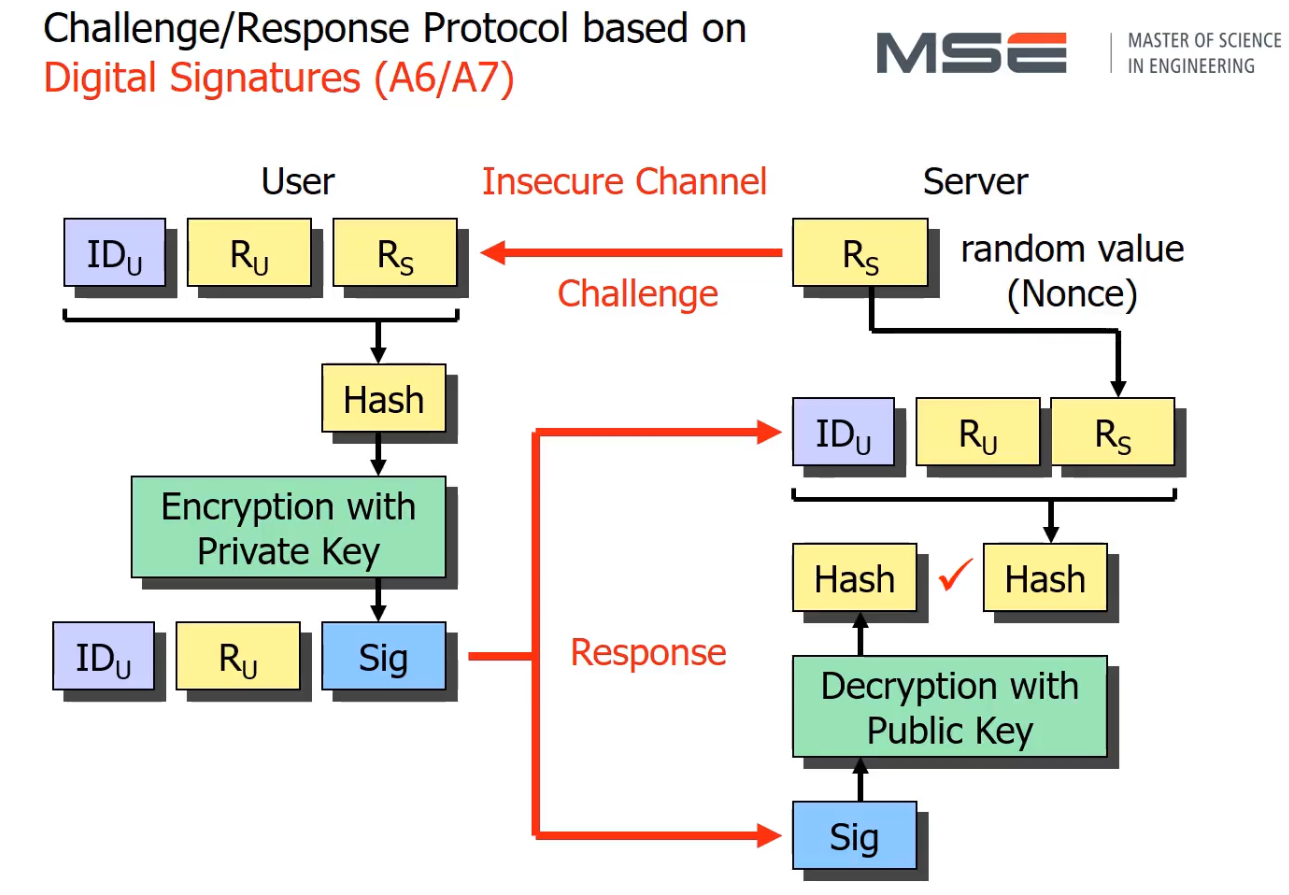
\includegraphics[width=\textwidth]{ChallengeResponseBasedOnDigitalSignatures.png}

\subsubsection*{Anonymous Key Exchange}
"Diffie helmann"

\begin{itemize}
    \item Can be used to create a secure tunnel to then use one of the previous methods
    \item vulnerable to MIM
    \item is Anonymous so you don't know if you are actually talking to a server
    \item requires quite a lot performance
    \item Has become the standard
\end{itemize}

\subsubsection*{A5 Zero Knowledge password proofs}
Uses "Diffie helmann" as well

\begin{itemize}
    \item Password database on both sides which can be stolen
    \item 
\end{itemize}

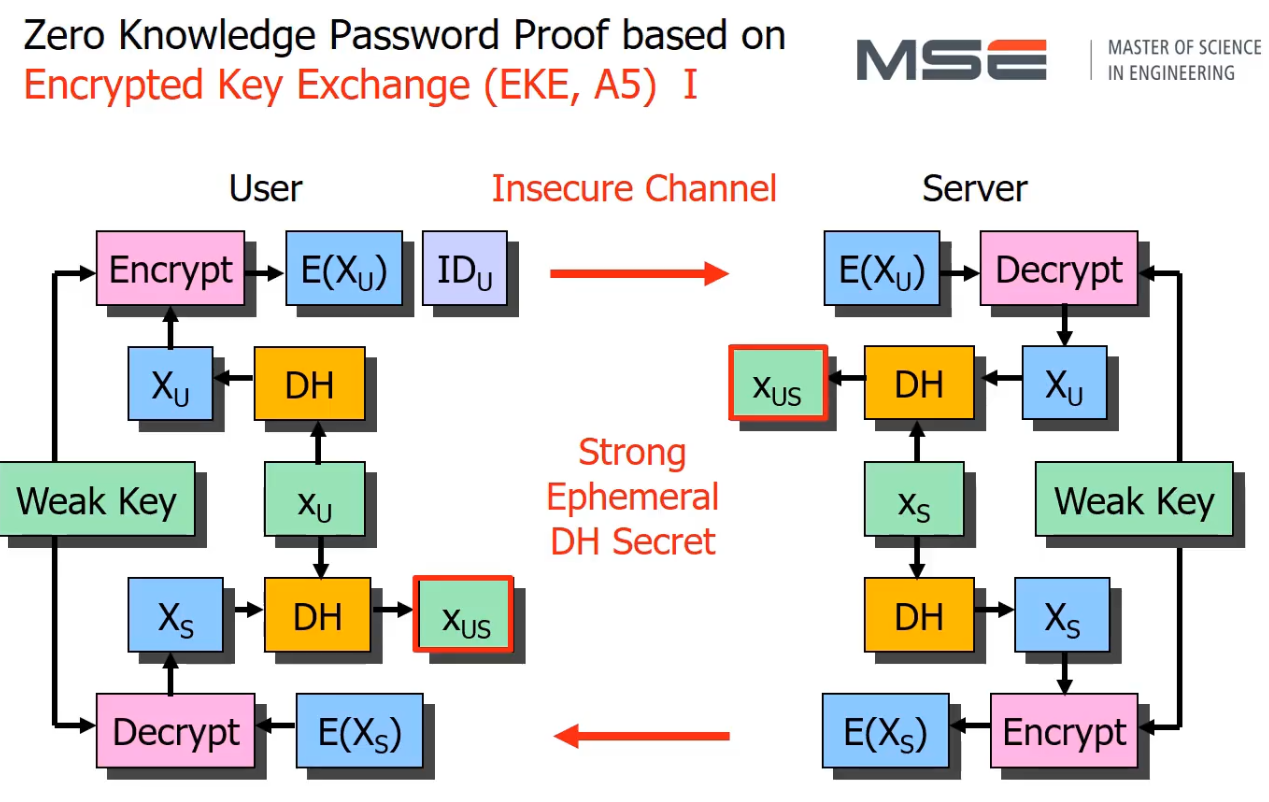
\includegraphics[width=\textwidth]{ZeroKnowledgePasswordProof.png}
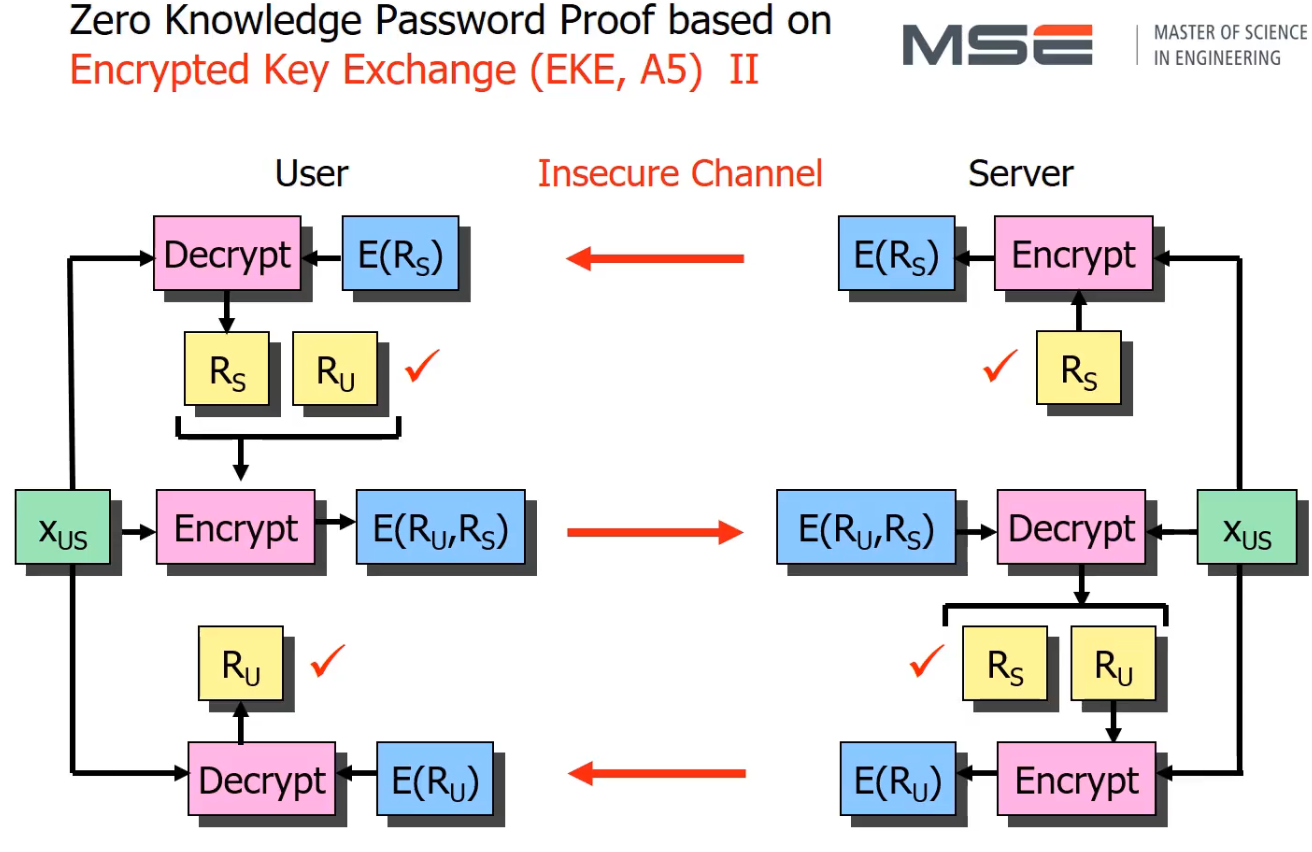
\includegraphics[width=\textwidth]{ZeroKnowledgePasswordProof2.png}
\subsubsection*{A6 Certificate-based server autentication}
"Diffie helmann" as well but with certificate

\begin{itemize}
    \item Can be used to create a secure tunnel to then use one of the previous methods
    \item If certificate trust chain is broken, MIM is possible
    \item Password list on server can be stolen
    \item Authenticates server and user
\end{itemize}

\subsubsection*{A7 Mutual public key authentication}
"Diffie helmann" as well to secure a channel

\begin{itemize}
    \item Certificates are transmitted throught tunnel.
    \item Each user needs a certificate which takes effort to handle.
    \item No user secrets on server, so no identity theft on server possible
    \item CA can be compromised
\end{itemize}

\subsection*{Practical Password lengths}
\begin{itemize}
    \item A...Z,0...9 = 36 symbols
    \item A...Z,0...9 = 62 symbols
    \item Printable = 95 symbols
    \item Length = 8 in 1sec/2min/55min
    \item Length = 10 30min/5days/347days
    \item Length = 11 18h/300d/90y
    \item Length = 12 27d/51y/8567y
\end{itemize}
Should be changed every 6 months, but forcing this may result in users building lists of password as they can't remember

\subsection*{Federated Identities}
\subsubsection*{The problem}
If for example a user needs access to ressources from different universities, without authentication & authorization infrastructure he needs different credentials for all universities

\subsubsection*{With authentication and authorization infrastructure}
An AAI layer is put between user and the universities
\begin{itemize}
    \item No registration with ressource necessary
    \item Uniform login procedure
    \item Opens up new resources to users
    \item Location independence
\end{itemize}

\subsubsection*{Shibboleth}
Shibboleth is an example for such a infrastructure

https://switch.ch/aai/demo

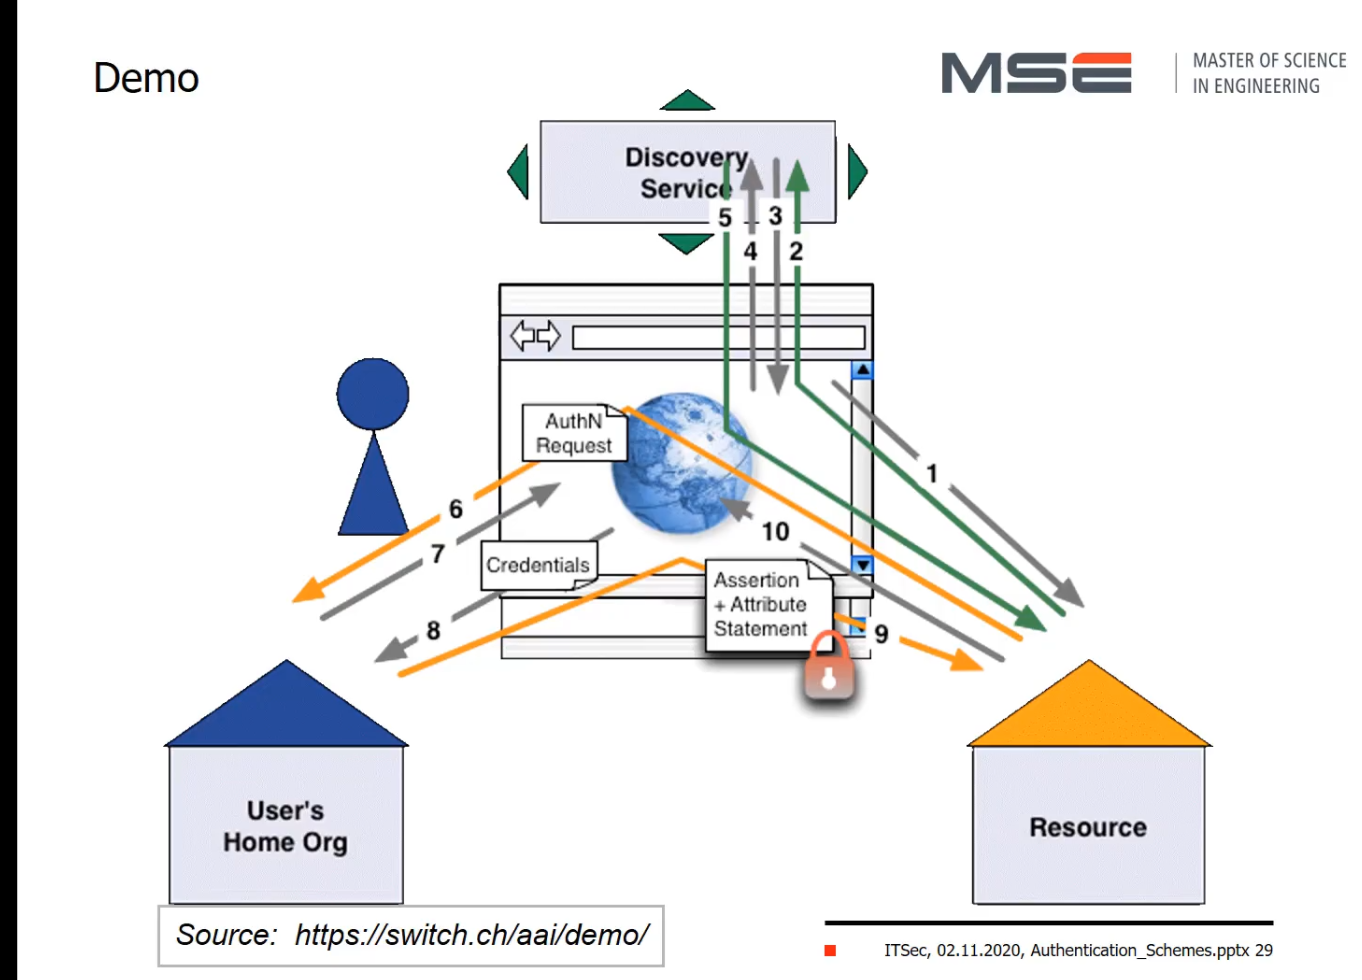
\includegraphics[width=\textwidth]{ShibbolethDemo.png}

Data is transmitted in xml defined in "XML Signature Syntax and Processing" and "XML Encryption Syntax and processing"

\subsubsection*{Secure Assertion Markup Language (SAML)}
XML-encoded assertions about authentication, attributes, and authorization (signed user credentials). Allows single sign-on solutions for web services

\subsection*{OAuth 2_0}
OAuth 2.0 consists of the following roles
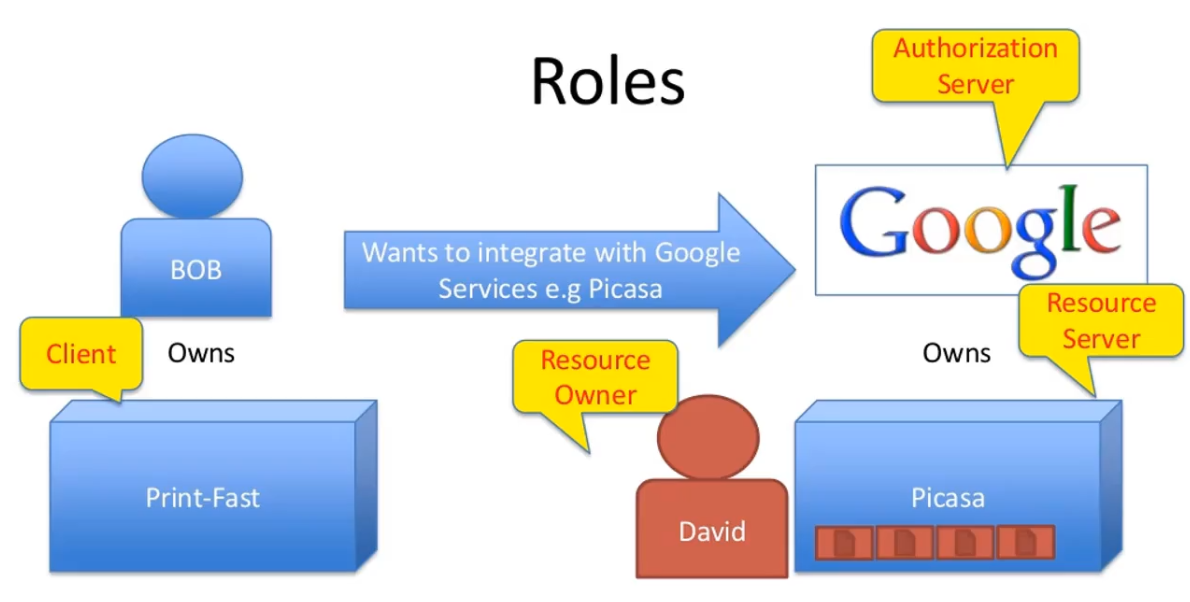
\includegraphics[width=\textwidth]{OAuth20Roles.png}

Passwords are never passed around in OAuth 2.0

https://youtu.be/CPbvxxslDTU

OAuth does not provide authentication as the access token is like an anonymous key

\begin{itemize}
    \item The application sends an authorization request to the authorization server
    \item This is in the form "Do you want to authorize the app ... to access ..."
    \item The Authorization will return n authorization Grant
    \item The authorization grant is used to request an access token from the authorization server
    \item The application can now access the requested ressources using the access token
\end{itemize}

\subsection*{OpenID Connect Authentication Layer}
OpenID Connect 1.0 is a simple identity layer on top of OAuth 2.0

https://youtu.be/Kb56GzQ2pSk

OpenID is for example used in SwissID

\section*{Access control}
\subsection*{Variants}
Example of access control in trains:
\begin{itemize}
    \item Preventive: For example sign in train: "You need a valid ticket or you will be fined"
    \item Detective: Controlleur will check validity of tickets in train.
    \item Corrective: Fine will be sent to users without a valid ticket.
\end{itemize}


\end{document}